\begin{figure}[htp!]
  \centering
  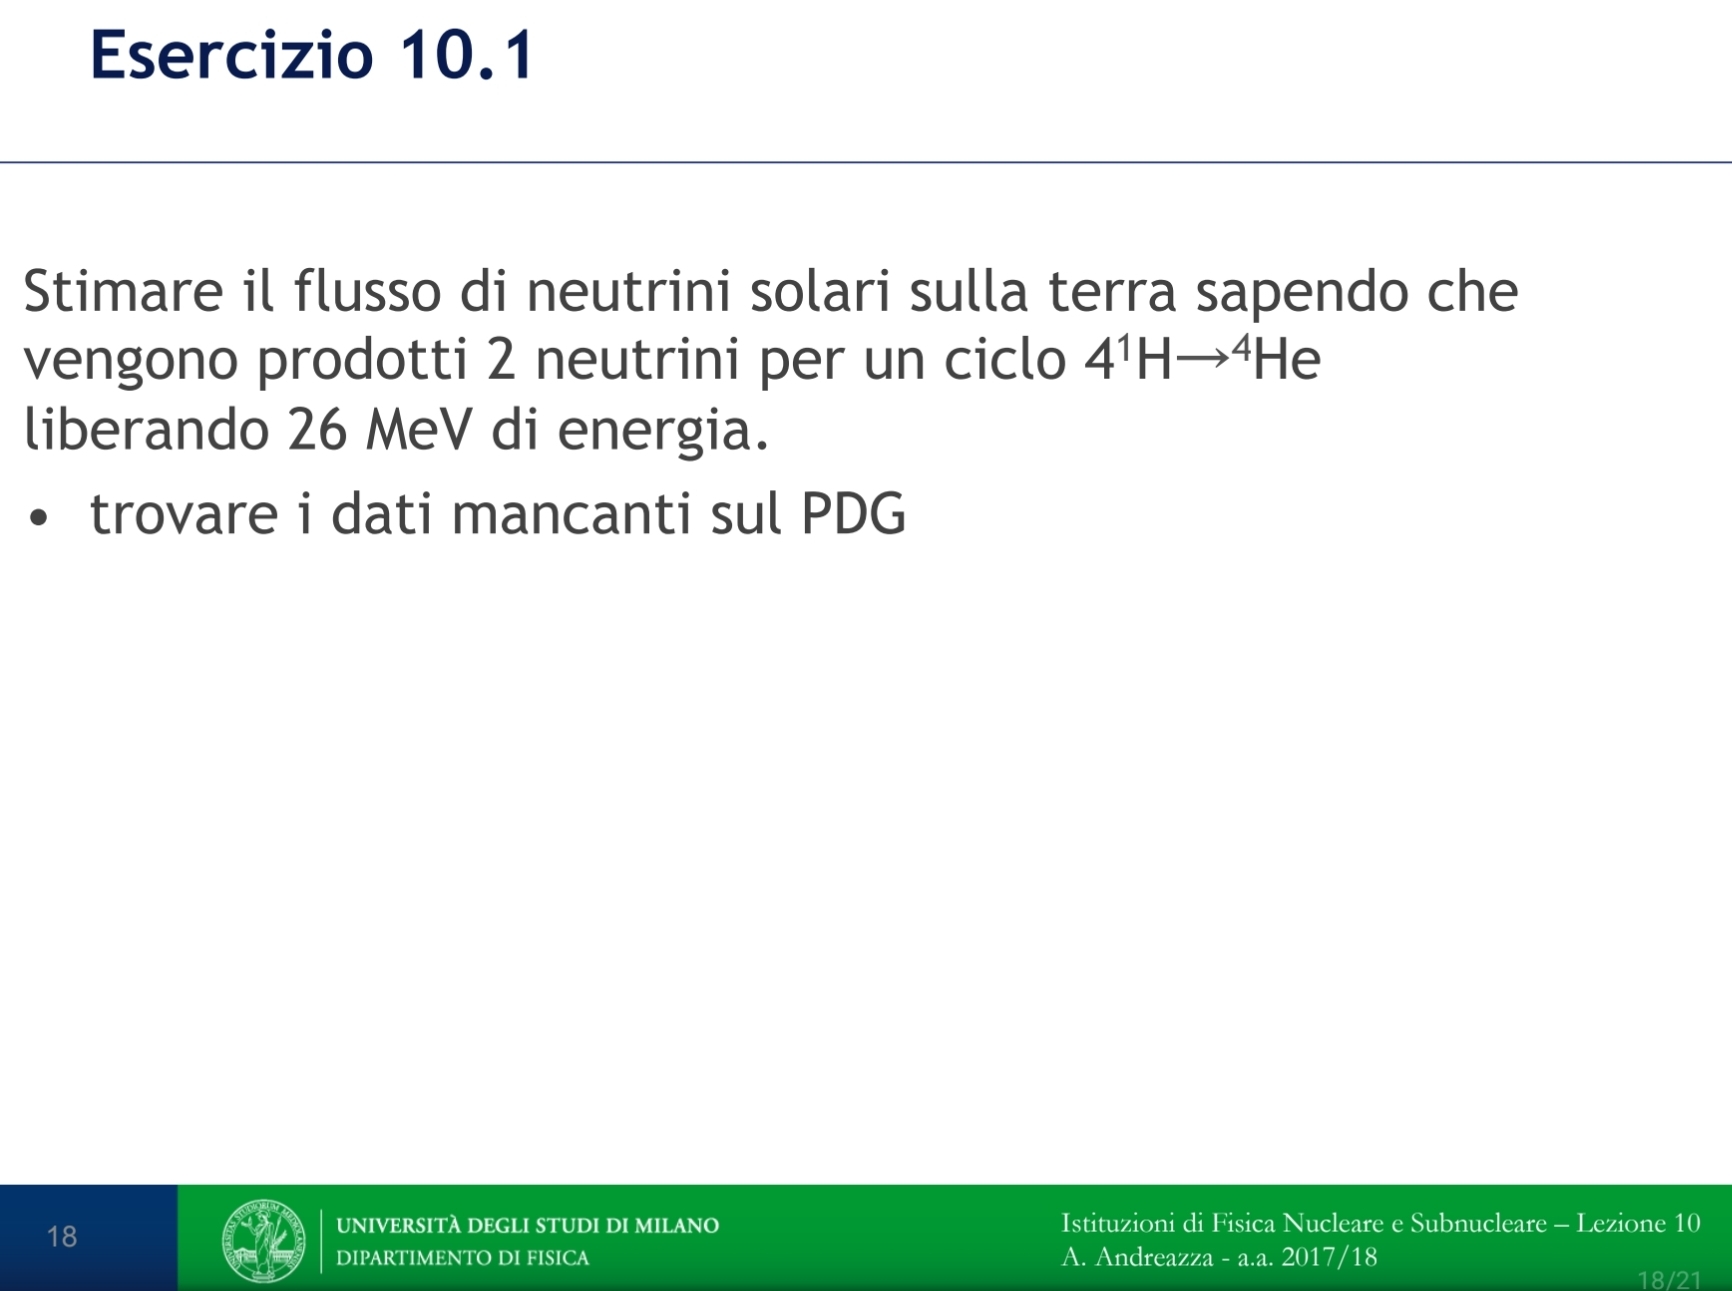
\includegraphics[scale=0.22]{Esercizio10.1/Esercizio.jpg} 
\end{figure}
Prima di tutto bisogna calcolare quanti cicli avvengono al secondo. Per fare questo è necessario conoscere la massa del sole: $M_{\odot}=2\cdot10^{30}\,\mathrm{kg}$ costituiti in massima parte da idrogeno. Grazie a questo è possibile calcolare il numero di atomi di idrogeno:
\begin{equation}
    N_H=M_{\odot}\frac{N_A}{A}=1.2\cdot10^{57}
\end{equation}
Conoscendo anche la potenza irraggiata dal sole: $L_\odot=4\cdot10^{26}\,\mathrm{W}$ è possibile calcolare il numero di cicli di fusione al secondo:
\begin{equation}
    \frac{dN_{\mathrm{fusioni}}}{dt}=\frac{L_\odot}{24.68\,\mathrm{MeV}}=10^{38}\,\mathrm{s}^{-1}
\end{equation}
Dove $24.68\,\mathrm{MeV}$ è l'energia liberata dopo un solo ciclo di fusione. Ogni ciclo di fusione produce $2$ netrini e quindi:
\begin{equation}
    \frac{dN_\nu}{dt}=2\cdot10^{38}\,\mathrm{s}^{-1}
\end{equation}
Il flusso dei neutrini si calcola:
\begin{equation}
    \Phi=\frac{dN_{\nu}/dt}{4\pi R^2}=8\cdot10^{10}\,\nu/\mathrm{cm}^2\mathrm{s}
\end{equation}
Dove $R=1.5\cdot10^{11}\,\mathrm{m}$ è la distanza della terra rispetto al sole.